\documentclass[10pt,twocolumn]{article}

% use the oxycomps style file
\usepackage{oxycomps}

% usage: \fixme[comments describing issue]{text to be fixed}
% define \fixme as not doing anything special
\newcommand{\fixme}[2][]{#2}
% overwrite it so it shows up as red
\renewcommand{\fixme}[2][]{\textcolor{red}{#2}}
% overwrite it again so related text shows as footnotes
%\renewcommand{\fixme}[2][]{\textcolor{red}{#2\footnote{#1}}}

%\DeclareUnicodeCharacter{2217}{∗}

% read references.bib for the bibtex data
\bibliography{references}

% include metadata in the generated pdf file
\pdfinfo{
    /Title (Reverse Engineering the GiantBomb API: Using Word Embeddings to Predict Video Game Recommendations)
    /Author (Yash Karandikar)
}

% set the title and author information
\title{Reverse Engineering the GiantBomb API: Using Word Embeddings to Predict Video Game Recommendations}
\author{Yash Karandikar}
\affiliation{Occidental College}
\email{ykarandikar@oxy.edu}

\begin{document}

\maketitle
 
\section{Introduction and Problem Context}

%This section should motivate why the project is interesting both to you and to the computer science community or the general public.
%You should also justify the difficult of the project.
%As a rough guideline, your project should be either narrow but deep in a subfield of CS, or broadly reaching across subfields without being too shallow.
%It should be comparable to the amount of work/content in an upper-level elective.

Working on this project is interesting to me because it provides an opportunity to combine machine learning (ML), natural language processing (NLP), and real-world data analysis into one problem. In terms of ML, I want to gain ML experience so that I can apply it in my career going forward (possibly in a healthcare-oriented context). Focusing on video games as the subject for the supervised machine learning problem has also allowed me to tap into an immense amount of text-based video game data (descriptions, reviews, and other qualitative aspects of online game discourse). In this way, I can use NLP techniques as ML features and apply them to a subject of interest. The real-world nature of this problem is also stimulating and challenging, because the data comes from an API that requires authentication and preprocessing. This is very different from the cleanly defined, open-access datasets used in my other courses. Combining ML, NLP, and real-world data modeling into one project has helped motivate my work in comps, and it has challenged me and helped me grow as a developer and machine learning researcher.

In terms of societal applications, recommender systems are critical to today's highly technological, choice-laden society. These recommender systems are found in many different aspects of life. Commercial websites (like Amazon \cite{AmazonRS}), video content platforms (YouTube \cite{YouTubeRS} and Netflix \cite{NetflixRS}), and social media websites (LinkedIn \cite{LinkedInRS}) are just a few examples. To help process data and provide recommendations, supervised learning (especially self-supervised variants of supervised learning algorithms) is often explored in the implementation of these recommender systems. Addressing data sparsity, alleviating the "cold start" problem of not having an initial suggestion to base future recommendations on, and including temporal aspects of recommendation as user sentiment changes are all good reasons to apply supervised or self-supervised learning. \cite{JYu, XXin, Matuszyk}

The difficulty of this project also stems from the machine learning side of the problem. Because common approaches for recommendation systems require immense amounts of user data and interconnected user profiles, they are not practical for the scope of this project. Instead, transforming the recommendation problem into a supervised learning problem creates an opportunity to practice real-world machine learning. Deciding which dataset I can use to provide ground-truth labels for recommendation is good practice, because real-world applications of ML often require extracting and preprocessing data from different sources in order to solve the question at hand. After obtaining the data, practicing iterative ML algorithm improvement - specifically identifying breakpoints and making changes to the algorithm to test out new hypotheses - has helped me gain a better perspective of how machine learning is conducted.

\section{Technical Background}

%This section introduces the technical knowledge necessary to understand your project, including any terminology and algorithms.
%You should assume that the reader is a CS undergraduate like yourself, but not necessarily familiar with AI/ML/HCI/apps/video games/etc.

Current approaches to recommendation systems use two main strategies, collaborative filtering and content-based recommendations. Content-based approaches examine how different entities connect together in qualitative ways. These recommendations typically cluster semantically similar products (especially when text-based descriptions are reasonable indicators of product appeal). One approach involves converting string queries (e.g., game titles like "Breakout" or "Tetris") or string content (game descriptions, reviews, and other corpora) into numerical vectors and comparing their contents to vectors of related games. The TF-IDF algorithm uses sparse numerical vectors (meaning that most vector elements are 0) to identify common keywords and penalize non-informatic keywords. Approaches that use it aim to find patterns of highly informatic, low-density word usage. \cite{Meidl, Zhang, DWang} Similarly, word embedding approaches such as Word2Vec \cite{Word2Vec} or the Google Universal Sentence Encoder \cite{SentenceEncoder} use dense vectors (with mostly non-zero vector elements) to compare similarity.

On the other hand, approaches that use collaborative filtering consider user similarity when linking together products. The key idea of collaborative filtering is to learn what product a customer likes, find related users in the database who like the same product, and use related users' profiles to generate suggestions for the customer. As an example, consider a user who shares that they like Super Mario Bros. Collaborative filtering examines other users in the database who also enjoy Super Mario Bros and recommends their enjoyed entries (perhaps The Legend of Zelda or Donkey Kong) to the initial user. The database thus needs to be data-dense enough to connect related users to the input provided by the initial user. Within industry, this data density requirement means that collaborative filtering is especially powerful in recommendation systems like Spotify \cite{JacobsonSpotify} which have a large, communicative user base. Collaborative filtering-based approaches are also standard in the literature. \cite{Chow, Ferdaous, PerezMarcos} Because of its ability to leverage the power of social networks for recommendations, collaborative filtering is a highly influential technique. Collaborative filtering is such a powerful idea that it can form a benchmark model for future improvements. \cite{Gohari, Ramzan} 

In both content-based approaches and collaborative filtering applications, recommender systems require large datasets (of products, users, or both) to effectively find connections between entities. Machine learning poses a way to process this immense data and identify patterns to form clusters, similarities, and eventually recommendations. Many types of machine learning techniques are applied to the recommendation problem. Supervised learning (where labels are known ahead of time), unsupervised learning (where the algorithm learns to cluster features by itself), and other approaches are also used. \cite{Nawrocka, XuAraki} Supervised learning algorithms are especially helpful in recommendation for a project of this scope, because answers are known ahead of time, so the focus can be improving the recommendation algorithm with respect to standard evaluation metrics rather than considering recommendation-specific evaluation metrics. Depending on the recommendation problem, different types of algorithms can be used.

In my comps project, the problem of recommendation is transformed from a collaborative filtering problem into a supervised learning problem. Because collaborative filtering requires millions of user profiles, any algorithm that uses collaborative filtering needs access to a robust user dataset. Instead, this project finds ground truth labels for recommendation from an online application programming interface (API) and builds a machine learning algorithm to perform well on the video game dataset. Thus, the problem turns from recommendation to \textit{reconstruction} of a recommendation algorithm using supervised learning. The problem is formulated as follows: Given an input game $g$, decide whether a potential recommendation game $r$ should be recommended.

To solve this supervised learning problem, the support vector machine (SVM) algorithm is used. SVM is a binary classifier, so it separates data points into two classes. SVM can create a linear or nonlinear decision boundary to differentiate the two classes. In this case, the kernel (the core that determines how SVM creates the decision boundary) is the radial basis function ("RBF") kernel. RBF is the standard for any nonlinear SVM classification. So, RBF-kernel SVM creates a nonlinear decision boundary between points of two classes (1s and 0s) such that distances from the margin are reduced as much as possible. \cite{CortesVapnikSVM} Cases with high class imbalances (where there are far more 0s than 1s, or vice versa) can be addressed by artificially creating similar points and adding those to the smaller class. \cite{NVChawla} The way that SVM is constructed combines optimal margin classification (reducing margin distances) and an efficient "kernel trick" which teaches the classifer how to map to nonlinear decision boundaries. By definition, the kernel trick helps SVM to work with high-dimensional data, which makes SVM particularly effective for problems that require high-dimensional inputs. \cite{Joachims, Berbatova} 

The input data to the SVM uses techniques from natural language processing (NLP) to transform textual data into numerical data that the machine learning model can use for training and testing. One possible NLP approach is to identify informatic words by topic modeling, where key ideas are extracted from a series of text documents and used as ML features. \cite{Ryan_51, Reuver} A related, but distinct, approach is to identify informatic words by context/through their syntactic structure \cite{Meidl, LDiCaro}. Another technique is to use word embedding vectors or matrix/tensor representations of word embeddings, where words are mathematically transformed from strings to floats and represented in N-dimensional space. \cite{Sifa_tensor} Many NLP approaches rely on powerful ideas from linear algebra to turn informatic text content into numerical machine learning features.

\section{Prior Work}

%This section describes of related and/or existing work.
%This could be scientific or scholarly, but may also be a survey of existing products/games.
%The goal of this section is to put your project in the context of what has already been done.

Prior work uses key ideas outlined in the technical background section as a foundation and strives to pivot or improve upon them. For instance, some approaches take collaborative filtering as a baseline and provide a more efficient, performant model. Others address limitations of collaborative filtering (the issue of \textit{only} considering user profiles) and limitations of content-based recommendation (the difficulty of gathering enough data to start the recommendation process) by combining them with other techniques. Many approaches display an interdisciplinary perspective by combining collaborative filtering with ideas from related fields (computational linguistics/NLP, ML, and so on).

Because of collaborative filtering's efficacy in the recommendation space, many approaches combine content-based methodology and non-social, numerical metrics with collaborative filtering models. Within industry, the Steam Interactive Recommender and Quantic Foundry \cite{SteamInteractiveRecommender, QuanticFoundryRecommender} generate
recommendations for a user $U$ by combining data-dense collaborative filtering techniques with non-social metrics that corroborate recommendation choices. For example, Steam looks at users who own similar games to $U$ in \textit{their} libraries, but it also looks at $U$'s user play time as an objective metric to see if $U$ actually enjoys their owned games. Similarly, Quantic Foundry combines collaborative filtering with profiles of gamer psychology - what motivates and interests players is a qualitative metric that further informs the collaborative filtering approach. Within the research world, collaborative filtering is often a benchmark model or baseline approach. Many approaches combine collaborative filtering with other analyses and hybrid methodologies. \cite{Choi, Gohari, PerezMarcos}

Interdisciplinary approaches using ML and NLP are also common because of their ability to apply various performant algorithms to the recommendation space. Machine learning algorithms like SVM can be tuned to delineate and output recommendation, which inspired part of this project's motivation. \cite{XuAraki} Because these ML algorithms are used to simulate recommendation, conventional ML metrics are used to evaluate the approaches \cite{Nawrocka, Chowdhury, Sujatha}. Similarly, NLP approaches appear in recommender systems as a means to categorize, extract, and recommend different entities. Content-based approaches that use categories like genre, theme, or sentiment as features can help classify the propriety of a potential recommendation. \cite{Berbatova, Asani}

A specific subset of ML and NLP approaches can help address the limitations of typical recommendation approaches. These limitations are primarily the difficulty of gathering enough information to start finding related items (the "cold start" problem). Any representation or data structure that can provide a qualitative feature (removed from quantitative metrics like similarity score, number of connections in the social network, etc.) is a potential improvement in performance. Some researchers turn to word embeddings as an answer. Combining word embedding content-based analysis with benchmark collaborative filtering obtains the best of both worlds from related users and products. \cite{LNguyen} Similarly, context-aware methods of word embeddings enhance typical content-based approaches (by considering context sensitivity, syntactic structure/relationships, etc.) and provide relationships between key words in recommendation corpora that can be informatic features in their own right, independent of the density of the database. \cite{CSundermann, Ramzan}. Such word embedding approaches are similar to the word embedding vector features used in this project. 

\section{Methods}

%This section describes what exactly you will be working on.
%What are you building? How will it combine/incorporate ideas from the literature? Be specific about what you will be doing: talk about the specific algorithm you will implement/use, the specific dataset/platform/API, and what the outcome of your project will look like.
%All of these decisions should be justified as well.

% The approach to the project is clearly laid out, and justified with respect to literature and the goals of the project. Alternate approaches and why they are not used are discussed.

\subsection{Problem Formulation}

I am reconstructing the GiantBomb API \cite{GiantBomb} (and specifically the GiantBomb similarity algorithm) by using a support vector machine algorithm trained on word embeddings of game descriptions. This reconstruction is what transforms the recommendation problem (should a game be recommended with respect to some initial input?) into a machine learning problem (does the algorithm output the correct label?) to solve.

The GiantBomb API acts as follows: given a query game $g$, it provides a set of similar games $S$. For this project, for every $s \in S$, $s$ is considered a valid recommendation for $g$. Conversely, for every $n \not\in S$, $n$ is not a valid recommendation for $g$. Using these definitions, the SVM algorithm can reconstruct the API output. 

Let $g$ be the query game, and let $r$ be a potential recommendation for $g$. Let $S$ be a set of similar games for $g$, obtained by $GB(g) = S$. Then the GiantBomb API's answer to the recommendation problem is to check if $r \in S$. If it is, the GiantBomb API is considered to return 1; else, 0. Similarly, the SVM's answer to the recommendation problem is to run $SVM(g, r)$, which gives a label 0 or 1. The performance of the SVM can then be measured by how well the SVM's labels correspond to the GiantBomb API's labels.

By using the GiantBomb API's labels as the ground truth data, training this supervised learning algorithm is the same process as training any other supervised learning algorithm. Thus, the problem statement is as follows. Given a query game $g$ and a potential recommendation $r$ as input, give output of whether the recommendation makes sense with respect to the query. Equations 1-3 display example runs of the SVM algorithm to illustrate sample inputs and outputs.

\begin{equation}
    recommender(g, r) = 1
\end{equation}

Eq. 1: r makes sense as a recommendation with respect to g.

\begin{equation}
    recommender("Tetris", "Breakout") = 1
\end{equation}

Eq. 2: Breakout makes sense to recommend if Tetris is the query game.

\begin{equation}
    recommender("Tetris", "Baldur's Gate") = 0
\end{equation}

Eq. 3: Baldur's Gate does not make sense to recommend if Tetris is the query game.

\subsection{Dataset}

Game titles were obtained from a combination of calling the GameSpot API \cite{GameSpot} and reading in the Metacritic CSV \cite{KaggleMetacritic}. The GameSpot API returned game titles, a collection of demographics (genres, themes, franchises), and text (sentence-long taglines called "deck" and longer-form paragraph called "description") as the response. The Metacritic titles were fed into the GiantBomb API to receive the same information. The query set $Q$ mapping titles to their demographics and text was then formed. When possible, titles were also mapped to their respective reviews (from the Metacritic CSV and GameSpot API) where they were available. Figure 1 provides a sample entry in the query set.

%\includegraphics[width=\textwidth,height=\textheight, keepaspectratio]{sample_input_.PNG}

% https://tex.stackexchange.com/questions/215708/fit-an-image-a-two-column-style
% https://www.overleaf.com/learn/latex/Questions/How_do_I_insert_an_image_at_a_specific_point_in_the_document%3F
% https://tex.stackexchange.com/questions/8625/force-figure-placement-in-text
% https://www.overleaf.com/learn/latex/Inserting_Images
\begin{figure}[h!]
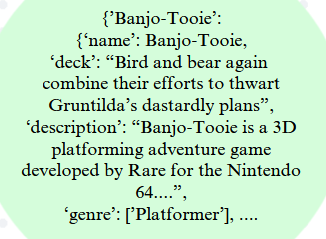
\includegraphics[width=8cm, height=6cm]{deck_desc_data_structure.PNG}
\centering
\caption{Sample entry in query set $Q$, mapping a game title to its text data and demographic categories}
\end{figure}

After forming the initial query set $Q$, the dataset for machine learning was built. For $g \in Q$, a set of similar games $S$ was obtained from the GiantBomb API (such that $GB(g) = S$). Every similar game $s \in S$ should be recommended (label 1). Similarly, every game $n \in Q$ where $n \not\in S$ should not be recommended (label 0). 

The tokenized words in the decks and descriptions of $g$ and either $s$ or $n$ were combined into one string. This string was converted into a word embedding vector, which formed the feature vector for the SVM. These vectors were mapped to the label (1 for $s$ and 0 for $n$). When reviews were available, adjective-context pairs were identified in the review text using dependency parsing. \cite{Meidl, LDiCaro} The words in the pairs were added to the combined string. So, the word embedding vectors of deck and description (and adjective-context pairs, when available) formed the features of the dataset, and the label was either 0 or 1 depending on the game similarity.

\subsection{Data Processing}
Data processing was conducted to smooth out the results. There were far more non-similar games than similar games, so synthetic minority oversampling was used to offset class imbalances. \cite{NVChawla} This technique generates points in N-dimensional space which are similar to the points already existing in the dataset. The goal is to balance the frequencies of the labels 0 and 1. For the SVM algorithm, dimensionality reduction was applied by principal component analysis. \cite{Joachims} Before fitting the SVM to the data, the dataset was projected from an N-dimensional space to a 2-dimensional space using linear algebra. This technique ensures that the decision boundary formed between the two classes is more precise.

\subsection{Algorithm}
For this experiment, SVM was used because of its ability to create a nonlinear decision boundary between the two classes. \cite{CortesVapnikSVM} It is a better choice for the task than other supervised learning algorithms like logistic regression, K-nearest neighbors, and tree-based models like random forest. 

By design, logistic regression deals with continuous data that has real-world, inherently meaningful implications. For example, logistic regression can be used to model housing prices given features of distance to the beach, highway, etc. This data is a real-world value (physical distance), so each data point has a meaningful physical representation. In this case, reducing distance to the beach may have a continuous, smooth increase in price. By contrast, the word embeddings used as feature vectors are not inherently meaningful, because they are numerical representations of words. So, a nudge in the word embedding vector values gives no intuition about how the word being represented might change, and it does not help in guessing similarity of different products the same way that a change in distance to the beach might help guess a change in housing price.

For K-nearest neighbors, the goal is to cluster together related entities by proximity. Using this model, given a game $g$, potential recommendations could be represented as points that are close to $g$ geometrically, and they could be evaluated by Euclidean distance. However, the problem at hand is not a problem of game similarity as much as a \textit{reconstruction} of the GiantBomb API. Because the API provides a list of similar games, the labels are less interesting than the process of reconstructing the process that provides the labels. As a result, an algorithm that determines similarity via inter-cluster distance is less necessary.

Finally, tree-based models like random forest often require enumerably many features that are determined before model training. The idea of random forest is to create partitions that isolate one part of the dataset at a time. For example, one partition in a random forest could be "distance from the beach", where a distance greater than a certain amount leads to a 0 label ("will not buy the house"). Every single partition in such a model is isolating certain cases. However, in this project, natural language is the key feature. The variability and density of natural language makes it hard to isolate numerical, meaningful features ahead of time, so random forest cannot find meaningful partitions to use.

Consequently, the SVM algorithm was the best choice for this specific use case. The algorithm was trained on the dimensionality-reduced dataset of word embedding vectors of deck/description. Figure 2 displays a sample X\_train and y\_train element. The list of word embedding vectors in the X array corresponds to the first label in the Y array. 

\begin{figure}[h!]
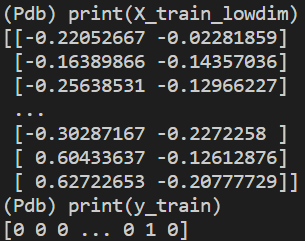
\includegraphics[width=8cm, height=6cm]{train_set_img.PNG}
\centering
\caption{Training dataset mapping word embedding vectors to labels}
\end{figure}

This dataset includes embeddings from both the query game $g$ and the potential recommendation $s \in S$ or $n \not\in S$. Word embeddings were chosen instead of TF-IDF because TF-IDF uses sparse word vectors (where a majority of vector elements are 0s). If sparse vectors are used, there are artificial positive matches between query game vectors and potential recommendation game vectors. This is because all vectors contain mostly 0s - there is overlap almost by definition. Such overlap leads to a non-discriminative classifier that is prepared to recommend everything. By contrast, word embeddings use dense word vectors, so game similarity can be constructed with respect to non-zero vector elements. 

\subsection{Hyperparameter Tuning}
Hyperparameters are parameters used in model training which can be adjusted to tweak performance. They are not fundamentally related to the dataset, but they do change some aspect of the model parameters which can slightly boost performance. 

The hyperparameter of interest for SVM is the C-value, which is inversely proportional to the tightness of fit around the decision boundary. How well does the model trade off between effectively fitting the training data and remaining general enough to fit the test data? A lower C-value means that the model has a better fit on the data, but it becomes more likely to overfit on test data. By contrast, a higher C-value means that the model has a worse fit on the data, but it becomes less likely to overfit on test data. The idea of tuning the C-value is to find the optimal point between a good fit and generality.

Accordingly, the C-value is a hyperparameter of interest. 5-fold cross validation is used to split the train/test data in 5 different ways so that C-values can be compared across models trained on different sections of the dataset. C-values of 1, 10, 100, and 1000 were compared.

\subsection{Outcome}
The desired outcome is a provided label (0 or 1) when a query $g$ and a potential recommendation $r$ are fed into the SVM algorithm. This outcome meets the goal of the project, because the idea is to use a supervised learning approach to reconstruct what the GiantBomb API would say. 

As stated in the problem formulation, the GiantBomb API takes a query game $g$ and returns a set of similar games $S$ in an operation $GB(g) = S$. A valid recommendation for $g$ is defined as $s \in S$. So, the GiantBomb API answer (0 or 1) to the recommendation problem can be determined by checking if the potential recommendation $r \in S$. 

As a result, running $SVM(g, r)$ simulates running $GB(g) = S$ and checking if $r$ is in the resulting set $S$. Since the SVM algorithm gives a label, that label is equivalent to running and checking whether or not $r$ should actually be recommended ($r \in S$). In this way, the SVM is able to reconstruct what the GiantBomb API says about game similarity.

\section{Evaluation Metrics}

%This section describes how you will evaluate your project.
%What will you be measuring, and how will you measure it?
%You might think about what would result in an F, a C, or an A for comps.
%Alternately, think about what are the minimal requirements for passing the class, what you might do if you had more time and resources, and what the best case scenario would be if everything went swimmingly.

% The metrics used and method of collection are clearly explained and justified with respect to the literature and the goal of the project. Other metrics and why they are not used are discussed.

The problem of interest has been turned from a recommendation problem (with standard approaches of collaborative filtering and content-based analysis) into a supervised learning problem. As a result, an immense amount of user data, preferences, and connections is no longer needed. To evaluate the methods, standard machine learning metrics can be used.

Even though the features for the machine learning model use word vectors of deck and description, cosine similarity is not applicable as a metric for the end result of the model. Cosine similarity is used frequently in the literature \cite{Ferdaous, Ryan_47, STata}, but it is primarily used in cases where natural language context is not considered. (For instance, a database search only requires string similarity between a query and an article - it does not necessarily need \textit{semantic} similarity beween the two tokens.) In other words, raw word counts and frequencies are the features rather than the semantics of the words themselves. Since the features for the SVM are primarily natural language, context (word order, syntactic structure, and parts of speech) still matter for effectively training the classifier. Cosine similarity would be applicable for a search engine-like tool (matching query strings to database strings), but it is less applicable for matching game descriptions to game descriptions.

Other standard metrics of recommendation systems are inapplicable because they measure good recommendation rather than good reconstruction. Some recommender systems evaluate results with respect to the user rather than with respect to an external set of ground truth data. Novelty, serendipity (a measure of unexpectedness and relevance for the user), and other such metrics are valuable when the evaluation considers whether the user likes the product. \cite{Cremonesi} For instance, scoring well on serendipity is a good sign for a system like Amazon \cite{AmazonRS} which wants to maximize profit by presenting new yet useful products to customers. However, the project focuses on reconstruction of the GiantBomb API rather than measuring how well users would like a recommendation $r$ given that they like a query $g$. This focus makes conventional ML metrics more relevant for evaluation.

Precision, recall, and F-1 score are all essential evaluation metrics for any supervised learning algorithm. \cite{NAlAzzam, Chowdhury, Sujatha} Precision calculates $\frac{TP}{TP + FP}$. Given that the model labels the instance as 1, how often is the model correct - how often is the recommendation $r \in S$? Recall calculates $\frac{TP}{TP + FN}$. Given that the label is 1 in actuality, how many 1s did the model accurately capture? More specifically, recall considers how many items $r_1, r_2, \dots, r_n$ were recommended by the model, given that $\{r_1, r_2, \dots, r_n\} \in S$. Finally, F-1 score is a metric that combines precision and recall. These metrics (which can be visualized with a confusion matrix) are valuable tools to understand how well the algorithm performs a trade-off between recommending all games it should and staying away from all games it should.

For a machine learning model in the recommender system domain, it makes sense to prioritize precision over recall. Precision involves the correctness of the overall recommendations. Given that the model labeled an instance as "recommend," how likely was that label to be true? Recall involves the correctness of the model in getting all instances that \textit{should} have been recommended - how many true recommendations did it miss? People have a finite amount of time for entertainment. This means that a) they cannot possibly consume everything, so missing out on a theoretically good recommendation is less important and b) their time means more in general, so the displeasure of a bad recommendation is higher. 

In addition to standard metrics of precision and recall, manual test cases are constructed and applied. These are not fundamental indicators of performance like precision, recall, and F-1 score, but they are informal, intuitive metrics which can indicate whether the model is leaning more towards precision or recall. Given an expectation of $SVM(g, r)$, does the test case conform to the expectation? Running these experiments allows for an informal assessment of whether the model errs on the side of high false positives (over-eager to recommend) or high false negatives (missing opportunities to recommend).

The minimum viable product for this project is a machine learning algorithm that outperforms random guessing. Assuming that the classes are balanced, an algorithm that always returns 1 will be correct 50\% of the time. Outperforming random guessing with an F-1 score greater than 0.5 is a benchmark that indicates basic satisfiability for the model. With more time and resources, the goal for the project would be a machine learning algorithm that is more performant (around 0.8 F-1 score). The best case scenario would be an algorithm that is highly performant (around 0.9 F-1 score, which is typically seen in the literature) and explainable (where test cases conform to intuition from several human volunteers interested in video game recommendation).

\section{Results and Discussion}

% The stated metrics are used and the results explained with respect to the methods. Alternate explanations and caveats to the results are explored. The results are connected to the goals of the project.

Table 1 displays the standard ML metrics for this project.

%\begin{table}
\begin{center}
\begin{tabular} { |c|c| } 
  \hline
  Precision & 0.825 \\ 
  \hline
  Recall & 0.697 \\ 
  \hline
  F-1 Score & 0.756 \\ 
  \hline
\end{tabular}
\end{center}
%\end{table}

Figure 3 displays a confusion matrix of true positives, false positives, false negatives, and true negatives. The idea of the confusion matrix is to show whether the model tends to focus on accurately recommending everything that it should (and also being too eager to recommend items it should have stayed away from) or whether the model tends to be correct (at the expense of missing items it should have recommended). In recommendation, it makes sense to emphasize precision over recall because the displeasure of acting on a bad recommendation outweighs the displeasure of missing good recommendations. 

\begin{figure}[h!]
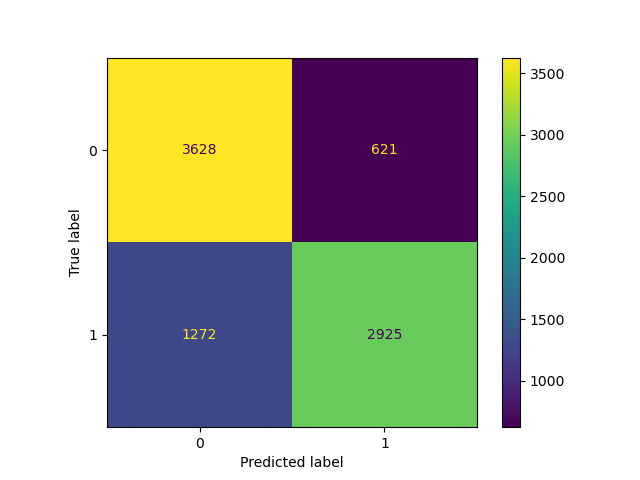
\includegraphics[width=8cm, height=6cm]{conf_matrix_visual.png}
\centering
\caption{Matrix illustrating trade-off between precision and recall (more TP implies more FP)}
\end{figure}

Figure 4 displays the test cases for recommendation. These are intuitive indicators of performance that provide insight into whether the model tends to be over- or under-eager to label specific games as 1 ("should be recommended"). Because most of the games are labeled as 1, the model captures most of the games it should recommend, but it also recommends games it should stay away from. This corresponds to the eagerness to label a product as 1 which makes sense for a recommender system. 

\begin{figure}[h!]
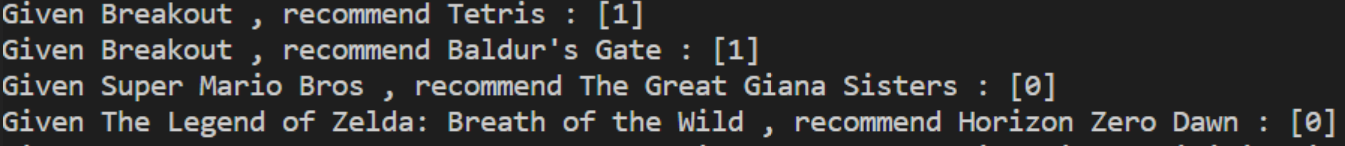
\includegraphics[width=8cm, height=2cm]{testcases_hyperparams_img.PNG}
\centering
\caption{Qualitative test cases to assess if model tends towards either precision or recall (keeping trade-off in mind)}
\end{figure}

The results of hyperparameter tuning were also applied to further improve performance. Since the RBF kernel was used to create a nonlinear decision boundary, hyperparameter tuning was applied to different C-values (1, 10, 100, and 1000) to compare relative performances. A new SVM was created and fitted using 5-fold cross validation to compare the C-values across 5 different iterations. In every iteration, C=1000 performed the best. Table 2 displays the F-1 score of each C-value for these different iterations.

\begin{center}
\begin{tabular}{ |c|c|c|c|c|c|} 
  \hline
  C=1 & 0.739 & 0.733  & 0.743 & 0.732 & 0.741 \\ 
  \hline
  C=10 & 0.743 & 0.739 & 0.747 & 0.737 & 0.748 \\ 
  \hline
  C=100 & 0.746 & 0.744 & 0.751 & 0.740 & 0.751 \\ 
  \hline
  C=1000 & 0.750 & 0.747 & 0.756 & 0.743 & 0.755 \\
  \hline
\end{tabular}
\end{center}

Overall, the results make sense given the methodology used in the experiment. Both the table and the test cases suggest that precision is greater than recall - false positive count is less than false negative count. This implies that the model tends to be accurate when it labels a game as "recommend," but it misses good recommendations that it could have provided. In addition to conforming to the expectations of a recommender system, the trend towards precision over recall makes sense given the use of natural language. The word embedding vectors of deck and description were key features in training the SVM. Because the algorithm is comparing possible recommendations through natural language features, it is more likely to recommend matches where the deck/description vectors between games have strong matches (higher precision). It is also likely to be conservative in what it recommends if the natural language input does not clearly indicate a match between query $g$ and recommendation $r$ (lower recall).

Even with lower recall than precision, the natural language features used to train the model capture much of the variability of the dataset. Just by feeding in word embedding vectors of deck and description, the model is able to accurately reconstruct the GiantBomb API to an F-1 score of 0.7. Being able to beat the baseline model just with text features implies that text (whether matter-of-fact descriptions, reviews, or perhaps even more emotive text found on forums online) is a valuable feature for predicting game similarity.

On the other hand, one of the limitations of the approaches used in this experiment is that natural language features may not only \textit{display} reduced recall, they may fundamentally \textit{imply} reduced recall. Even if two games have the same demographics (genre, theme, and franchise), the way in which they are described in their deck and description supersedes any demographic connection two games may have. This hesitance to connect two games purely on demographics means that the model will have less positive labels (1s) in favor of negative labels (0s), thus increasing precision at the cost of recall. For example, consider recommending the first Super Mario Bros game given the original Donkey Kong arcade game. The genre (platformer) and franchise (Mario) are the same, but the descriptions may very significantly ("famous, influential arcade game" vs. "blockbuster home console video game"). In this way, an algorithm trained purely on word embeddings will miss what is otherwise an accurate recommendation. 

To address this limitation, other NLP approaches like dependency parsing or sentiment analysis can be applied. \cite{Ryan_47} Addressing cases where demographics are similar but descriptions are different with sentiment analysis can help improve performance. For example, suppose Gran Turismo is posed as a recommendation for Mario Kart. If the descriptions for both discuss similar driving physics, the social nature of the gameplay, and so on, the algorithm can apply NLP techniques (e.g., connecting adjectives to nouns) to see if the embeddings for \textit{those} natural language strings are more similar. \cite{Meidl} In this way, NLP techniques can reveal similarities which unedited text did not show.

In general, the results meet the goals of the project. Because $SVM(g, r)$ simulates running $GB(g) = S$ and checking if $r \in S$, it provides the desired output. The SVM captures much of the variability of the GiantBomb API labels using this approach, so it is an appropriate reconstruction algorithm for the API. 

\section{Ethical Considerations}

%Are there any ethical concerns that might arise from your project?
%You might think about whether your project perpetuates societal inequity (or could be used by others to do so), whether the data/platforms you are using is collected with informed consent and free of bias, and whether you might be subject to technological solutionism instead of working support/better the public infrastructure.
%Include a discussion of how you plan to mitigate these issues in your project.

Any machine learning project is subject to ethical considerations which need to be addressed. Because this project uses machine learning to reconstruct the GiantBomb API, mitigating data bias is essential. Furthermore, any project that uses natural language, free-text data needs to consider how to moderate and mitigate abusive content if it is found.

Like any machine learning project, the model is only as good (or as biased) as the data on which it is trained. The SVM algorithm is trained on data from Metacritic, GameSpot, and GiantBomb. For the deck and description, the text data comes from verified reviewers who have write access to those websites. This content is less likely to be subject to bias, because it is a matter-of-fact text corpus that summarizes the content of a video game without opinion. However, variability among reviewers who write decks and descriptions may be an issue. This is addressed in future work.

For the review data, average video game players can submit review content. This content has more of a likelihood to skew the model because of "edge cases" like irony, misinformation, and speaker intention. \cite{Vidgen} To address this possibility, multiple different sources were used instead of only using the GiantBomb API.

Abusive content in the free text reviews is also a possibility. Any application which uses natural language as a feature or output possibly has to contend with abusive content, which includes (but is not limited to) hate speech, casual racism/sexism/other discrimination, etc. Care has to be taken to make sure that this sort of speech is not learned and casually amplified by the model. With more time, one way to check for this would be to use common methods of removing hate speech from the dataset. One way to do so is to perform a search to ensure that any provided input string is not found within a centralized, curated hate speech dataset. \cite{Mathew} This is not currently implemented, but is an important direction of future work. As important as moderation is, however, it is less necessary in a project like this where data is obtained from websites that are about game \textit{content} rather than game \textit{discussion}. For example, GameSpot has lots of news about game news, development, updates, and so on, but it has less activity in forums where users congregate. By contrast, forums such as Reddit which have more game \textit{discussion} are more likely to be vectors of this abusive content. This means that abusive content is less likely to be obtainable in this project, but it is still worth considering and implementing if more time was available.

\section{Future Work, and Conclusion}

Future work can improve the model performance by ensuring that the model does not propagate bias further in its output. In terms of ethical considerations, future work includes using standard approaches of abusive content detection \cite{Mathew} to process such content as needed. Even without ethical considerations, the way in which decks and descriptions are written is still subject to variability. Even amongst the same API, different authors may have written the text items in different ways, and this introduces a new layer of complexity. Future work could mitigate this uncertainty by getting deck and description elements for each game from different APIs (rather than just one API per game as in the current architecture). 

Model training is another area where future work can continue to improve performance. Currently, word embedding vectors of deck and description are the influential features used to train the SVM algorithm. Future work could include dependency parsing approaches on different sorts of text to get a better sense of syntactic structure. \cite{LDiCaro} Instead of only considering adjective-noun pairs, further grammatical structure (adverb-verb pairs, other dependency tags, etc.) could be explored. Other features of sentiment analysis could also be used; topic modeling, sentence polarity, and other feature extraction methods could also potentially improve performance. \cite{Ramzan, Ryan_51} Any NLP method that focuses on extraction or identification provides informatic features for the model to train on to further contextualize its word embedding focus.

\appendix

\section{Replication Instructions}
% All software used by the project is listed, with instructions that successfully allow another CS student to execute it. Particular attention is paid to future-proving the instructions (eg. package version, VMs, etc.)

\subsection{Software Used}
Key software used by the project is listed below.

\begin{itemize}
\item spacy=3.7.2 (for dependency parsing analysis of adjective/context word pairs)
\item tensorflow=2.14.0 and tensorflow-hub=0.15.0 (setting up the TensorFlow Universal Sentence Encoder for word embedding vector generation)
\item imbalanced-learn=0.11.0 (performing synthetic minority oversampling to offset class imbalance)
\item pandas=1.5.3 (setting up DataFrames)
\item numpy=1.25.0 (using numpy arrays for word embedding data types)
\item scikit-learn=1.2.2 (for the SVM algorithm, pipeline, evaluation, etc.)
\end{itemize}

\subsection{How to Run}

% https://www.overleaf.com/learn/latex/Hyperlinks
\begin{itemize}
    \item obtain API keys from \href{https://www.giantbomb.com/api/}{GiantBomb} and \href{https://www.gamespot.com/api/}{GameSpot}
    \item navigate to a directory on your computer, and run: 

    \begin{lstlisting}
    git clone https://github.com/y0shK/comps-video-game-recommender.git
    \end{lstlisting}
    
    \item create .env in the same directory as recommendation.py by using the following command:

    \begin{lstlisting}
    touch .env
    \end{lstlisting}
    
    \item put API keys into .env
    \item download metacritic\_game\_info.csv and metacritic\_game\_user\_comments.csv from \href{https://www.kaggle.com/datasets/dahlia25/metacritic-video-game-comments}{Kaggle}, and put both files in same directory as recommendation.py
    \item create conda environment in the same directory
    \item run:
    \begin{lstlisting}
    conda create --name YOUR_ENV --file requirements.txt
    \end{lstlisting}
    \item run:
    \begin{lstlisting}
    python recommender.py
    \end{lstlisting}
\end{itemize}

\section{Code Architecture}
%The code is organized logically, with comments on complicated algorithms. The organization of the code is clearly laid out/diagrammed, with justification. Another developer could use the overview to extend or debug the project.

%The code is split up into three main parts; dataset, algorithm, and postprocessing/data exploration. 

\subsection{Dataset}

\subsubsection{Initial setup}
Relevant imports are made (as described in the Replication Instructions section). For the data, a requests\_cache session for API calls is created and CSV files for Metacritic data are read in. A web model for Spacy dependency parsing through adjective/context word pairs is also instantiated.

\subsubsection{Data collection}
From the CSV titles, game titles are mapped to reviews, deck/description, and demographic information. This hash table of reviews is joined with API call data (from GameSpot and GiantBomb) to form the query set of data, and reviews are also mapped to when available.

\subsubsection{Dataset collation}
The TensorFlow Sentence Encoder is set up for word embedding generation. Iterating through the query set, the query game $g$ is mapped to every possible recommendation $r$. The API is called to generate $S$, where S is a set of "similar games" to $g$. Then checking if $r \in S$ maps the word embedding vectors of deck/description for both $g$ and $r$ to 0 (not similar) or 1 (similar). Adjective-context word pairs are also found using Spacy dependency parsing, and key words of adjectives and their respective nouns are fed into the string that is converted to a word embedding. If reviews are present in the current $g$ or $r$, they are tokenized and added to the string before word embedding as well.

\subsection{Algorithm}

\subsubsection{Synthetic minority oversampling}
To offset the class imbalance, synthetic minority oversampling \cite{NVChawla} is used to generate similar points in N-space. Upon resampling, the data is shuffled to prepare for training.

\subsubsection{Training}
The dataset is split into train and test sets with an 80-20 split. An SVM instance is created by using principal component analysis so that the decision boundary is simpler. The SVM model is trained on the train set.

\subsubsection{Evaluation}
The SVM model is evaluated on the test set. A confusion matrix is generated to visualize the tradeoff between precision and recall.

\subsection{Postprocessing}

\subsubsection{Data exploration}
Hyperparameter tuning is conducted by creating a new SVM classifier and varying C-values. 5-fold cross validation is used and results are compared. Test cases are executed and visuals are created to get a sense of the demographic characteristics of the dataset.

\printbibliography
\end{document}

